\documentclass[a4paper,12pt]{article}

\usepackage[margin=2.5cm]{geometry}
%\usepackage{mathpazo}
\usepackage{amsmath,amssymb}
\usepackage{graphicx}
\usepackage[usenames,dvipsnames]{color}
\usepackage{float}
\usepackage{colortbl}
\usepackage{amsthm}
\usepackage{units}
\usepackage{mathabx}
\usepackage{hyperref}
\usepackage{xspace}
\usepackage[noend]{algorithmic}
\renewcommand{\to}{\textbf{ to }}
\changenotsign

\usepackage{multirow}
\usepackage{natbib}
\bibliographystyle{elsarticle-harv}

\definecolor{DarkBlue}{rgb}{0.00,0.00,0.55}
\hypersetup{
    linkcolor   = DarkBlue,
    anchorcolor = DarkBlue,
    citecolor   = DarkBlue,
    filecolor   = DarkBlue,
    pagecolor   = DarkBlue,
    urlcolor    = DarkBlue,
    colorlinks  = true,
    pdftitle    = {Numerical Methods 1},
}


\definecolor{paleblue}{rgb}{0.9,0.95,1.0}
\definecolor{palegrey}{rgb}{0.9,0.9,0.9}

%\renewcommand{\chaptername}{Lecture}
\newcommand{\CDPA}[1][]{Copyright, Designs and Patents Act 1988 #1\xspace}
\newcommand{\SD}[1][]{Software Directive #1\xspace}
\newcommand{\Berne}[1][]{Berne Convention #1\xspace}

\usepackage[T1]{fontenc}
\usepackage[sc]{mathpazo}
%\linespread{1.05}


\setlength{\parskip}{2ex}
\setlength{\parindent}{0ex}


\begin{document}

\title{Principles of copyright in software}

\author{Dr David Ham}

\renewcommand{\today}{24 May 2013}

\maketitle

\section{What is copyright?}

Copyright is a set of \emph{legal property rights}\ which the author of a work, or
their employer, is granted by statute. These allow the copyright owner to
control certain acts in relation to that work. The original intention of copyright
law is to allow owners to generate income from their works by acts such as
selling copies. As we shall see, the rights granted by copyright statutes
can also be used to control the use of works in other ways.

\section{The legal basis of copyright}

Copyright is a statutory right created in UK domestic law by legislation
passed by parliament. The current copyright act in the UK is the Copyright
Designs and Patents Act 1988. However copyright exists in a wider context of
European and international law. This creates a system of copyright law which
is much more internationally uniform than is the case for other domains of
law such as contract, tort\footnote{Tort is the technical legal term for
  private law matters such as negligence, trespass and the civil (but not
  criminal) aspects of assault.} and criminal law. This means that most of
what we will cover in these lectures will hold true in many other
jurisdictions. Attempts will be made to highlight important international
differences, especially between the situation in the EU and that in the US.

Some of the more important international sources of copyright law which
affect the protection of computer programmes are:
\begin{description}
  \item[Convention for the Protection of Literary and Artistic Works]
    otherwise known as the Berne convention. This dates back to 1886 and
    establishes such basic principles as recognition of copyright in works
    authored overseas, and sets out an international minimum term of
    protection of the life of the author plus 50 years.
  \item[Directive on the Legal Protection of Computer Programs (the Software
    Directive)] Directive
    2009/24/EC  is the current piece of EU legislation
    extending copyright to computer programmes. It details the key rights of
    copyright holders, but also extends particular rights to legal users of
    software.
  \item[Information Society Directive] Directive 2001/29/EC harmonises 
    copyright more generally, but has particular provisions which are
    germane to computer programs. In particular, this directive requires
    member states to prohibit the circumvention of technological access
    controls and copy protection of work covered by copyright. In the UK
    this has been implemented in sections 296-296B of the Copyright Designs
    and Patents Act 1988. Another important exception to copyright
    introduced by the Information Society Directive was for temporary copies
    produced for technical reasons. This placed on a more secure legal
    footing activities such as web caches and the copying of information
    which occurs automatically as it moves around computer systems.
\end{description}

\section{Copyright as intellectual property}

It might sound strange at first hearing to hear copyright described as a
property right. We're used to the concept of property rights, or ownership,
in land or in physical objects, but what does it mean to say that a
statutory bundle of rights like copyright is a form of property? 

To understand this, we need to understand what distinguishes property rights
from other legal rights under, for example, contract law or in tort. There
are some defining features of property law which we can recognise in
copyright:
\begin{enumerate}
\item Property rights are enforceable against any third party without that
  party's consent. This is true
  for real property: the owner can generally exclude any third party from
  his or her land, and it's true for copyright: in general all third parties
  are subject to the exclusive rights of the copyright holder. Conversely,
  if Alice enters into a contract with Bob, then Charlie is unrestricted by
  any of the obligations in that contract.
\item Property rights are alienable: they can be transferred in whole or
  part to other parties. This is true for copyright as well, and the
  transferee then enjoys the rights on the same basis as the original
  holder.
\item Property rights can be waived in part by the granting of licences. I
  waive my right to sue you for trespass by inviting you onto my
  land. Similarly, the copyright holder may grant licences to copy,
  distribute, or otherwise deal in copyright works, and a licensee does not
  breach copyright law by acting in accordance with that licence.
\end{enumerate}

It is important, however, not to take this analogy beyond its scope. A good
example of this is theft. Theft is a very particular criminal offence
concerned with dishonestly making off with personal property. It is simply
not possible to commit this crime with respect to a set of immaterial legal
rights. Violating copyright can in some cases be a criminal offence, but it
will be an offence under the Copyright Designs and Patents Act 1988 and
unrelated to the offence of theft created by the Theft Act 1968. 

\subsection{Other forms of intellectual property}

Copyright is not the only form of intellectual property, nor is it the only
one which can affect software. However copyright is the form of intellectual
property which affects all developers and users of software most
pervasively. These are some of the other forms of intellectual property
which impact on software but which are beyond the scope of these lectures.

\begin{description}
\item[Trademark] trademark law restricts the use by third parties of the
  distinctive names and logos associated with products, including software.
\item[Patent] protects the ideas behind inventions. In Europe, software
  \emph{per se}\ is not patentable but software which causes physical
  effects may be patentable as a part of an invention. In the US, a much
  broader class of software is patentable.
\item[Database rights] are \emph{sui generis}\ rights in the collection of
  data together to form a database.
\item[Design rights] protect the design of objects from copying. These are
  not directly relevant to software development but can be relevant to
  graphical designs implemented in software, for example for fonts.
\item[Topography rights] are \emph{sui generis}\ rights in the design of
  semiconductors. These are of relevance to hardware designers.
\end{description}

\subsection{Your programme is a book}

Copyright applies to far more than software: books, art work, music, and audio
and video recordings are among the categories of work which attract the
protection of copyright law. The rights associated with copyright vary
somewhat according to the class of work so it's important to know to which
one your output belongs. Computer programs are quite a lot newer than most copyright
law, and so were slotted in later. Computer programs (in both source and
object form) are considered to be literary works for the purpose of
copyright protection\footnote{\SD[art 1]; \CDPA[s 3]}. However as we shall
see below, recent legislation, particularly the \SD, has created
rights and limitations which are peculiar to computer programmes and do
not, for example, apply to books.

\section{The rights granted by copyright}

The essence of copyright law is the granting to the copyright holder of
certain exclusive rights, or monopolies, in the copyright work. These rights
belong exclusively to the copyright holder and, subject to only limited
exceptions, everyone else requires the copyright holder's permission to do
any of these things.

\begin{enumerate}
\item The right to make copies whether permanent or temporary, in particular
  this includes those copies required to load, display and run the program.
\item The right to translate, adapt, arrange or otherwise alter the
  program. In particular this includes compiling, decompiling and translating
  into another programming language.
\item The right to distribute to the public, including renting copies of the
  program.
\end{enumerate}

These rights are laid out in article 4.1 of the Software Directive, and in
sections 16-21 of the \CDPA. 

In addition to these primary rights, there are a number of secondary
restrictions imposed by copyright law concerned with matters such as dealing
in infringing copies. We will not consider these matters here.

\subsection{Exceptions to copyright}

Articles 5 and 6 of the Software Directive lay out several 
exceptions to the exclusive rights of the copyright holder. Some of these
can be really important to the software developer.

\begin{description}
\item[The right to use] In the absence of specific contractual
  (i.e. licence) terms to the contrary, someone with a lawfully acquired
  copy of a piece of software is entitled to use it for its intended purpose
  and any copies made in the course of this (such as when the program is
  loaded into RAM) will not infringe copyright. This even extends to
  modifying the program to correct errors.
\item[The right to make a backup] Someone with the right to use a piece of
  software is also entitled to make a backup copy where that is necessary
  for the use. This is quite a limited right.
\item[The right to observe, study and test] ``The person having a right to
  use a copy of a computer program shall be entitled, without the
  authorisation of the rightholder, to observe, study or test the
  functioning of the program in order to determine the ideas and principles
  which underlie any element of the program if he does so while performing
  any of the acts of loading, displaying, running, transmitting or storing
  the program which he is entitled to do.''\footnote{\SD[art 5.3]} This
  right would appear to enable the use of debuggers and other monitoring
  tools.
\item [The right to decompile] In limited circumstances, it is legal to copy
  and translate an otherwise legally held copy of a piece of software in
  order to achieve interoperability with an independently created piece of
  software. This right is restricted to those actions needed to achieve
  interoperability, and the relevant information must not be readily
  available.
\end{description}

The right to use is essentially a default term in every software licence
which may be modified in the licence (for instance to prohibit commercial
use of software). The other rights in this
section hold for all legal users of software \emph{even if the software
  licence says otherwise}. This is required by \SD[art 5] and is implemented
by \CDPA[ss 50A-50C \& 296A].

\subsection{The term of copyright}

Copyright law is usually described in terms of a trade-off in which authors
are encouraged to produce works by the economic benefits they can derive
from the copyright in those works, and in return the works will eventually
become freely available to all of society. However, the Berne Convention
requires a copyright term of the life of the author plus 50 years\footnote{\Berne[art 7]}, and EU
law now requires that copyright last for the life of the author plus 70
years.\footnote{Council Directive No. 93/98/EEC Harmonizing
  the Term of Protection of Copyright and Certain Related Rights 1993 art
  1.}. In the case of a work of joint authorship, the duration is measured
using the death date of the last surviving author. The effect of these terms
in the fast-paced and young field of computer programming is that copyright
is, for practical purposes, permanent. To provide some perspective, any
surviving computer programmes written by Alan Turing will remain protected
by copyright until 2024.

The current long terms of copyright are the result in no small part of
extensive lobbying by large commercial copyright owners, typically from
fields outside computer programming. The extensive role played by one
particular US company in lobbying for the US Copyright Term Extension Act 1998 (also to
life plus 70 years) led to opponents terming that law the ``Mickey Mouse
Protection Act''.

\subsection{Who owns copyright in a work?}
 
Ownership of copyright in a work is governed by \CDPA[s 11], a piece of
legislation which is so unusually clear that it is convenient to reproduce
the first part of the section here verbatim\footnote{The remaining subsection relates to works by public
  bodies and is not relevant here.}:
\begin{enumerate}
  \addtocounter{enumi}{10}
\item First ownership of copyright. 
  \renewcommand{\labelenumii}{(\arabic{enumii})}
  \begin{enumerate}
  \item The author of a work is the first owner of any copyright in it, subject to the following provisions.
  \item Where a literary, dramatic, musical or artistic work, or a film, is
    made by an employee in the course of his employment, his employer is the
    first owner of any copyright in the work subject to any agreement to the
    contrary.
  \end{enumerate}
\end{enumerate}

Since students are not employees, copyright in anything a student writes
belongs to the student personally. Some universities have copyright policies
which claim ownership of their students' work. In the light of the above
legislation, it is very unclear on what basis these policies purport to operate.

\subsection{Copyright applies automatically}

It is very common to hear people use the word ``copyright'' as a verb, and
to hear about whether certain works ``have been copyrighted''. This is based
on a fundamental mistake about copyright law which may be rooted in a
confusion with patent law (for which registration is a
requirement). Copyright exists in a literary work, including a computer
program, as soon as it is recorded in writing or otherwise\footnote{\CDPA[s
  3.]}. For computer programs, this means that copyright exists in the
source code from the moment it is typed into the computer, and copyright
exists in object code the moment it is written out from the compiler. 

\subsection{Penalties and remedies for violation of copyright}

Breaching any of the exclusive rights granted under copyright law is a
statutory tort which may be enforced through the civil
courts\footnote{\CDPA[s 96]}. The remedies available include damages or an
injunction, for example prohibiting further distribution of infringing
copies. There are, in addition, several remedies, such as an order to
deliver up the infringing copies, which are particular to copyright
infringement\footnote{\CDPA[ss 96-100]}. From the perspective of a software
startup, the costs of litigation for breach of copyright could themselves be
severely problematic, and an order to cease distributing a product which
infringes copyright could be ruinous.

In addition to the civil remedies available to copyright holders, deliberate
copyright infringement in the course of business or at large scale can be a
criminal offence punishable by fines or imprisonment\footnote{\CDPA[s 107]}.

\section{The scope of copyright in software}

From the perspective of the software developer, there are several important
questions about the scope of copyright law and what actions by a developer
might infringe copyright. The extent of copyright coverage in software is a
matter of interpreting the legislation, a task which falls to the courts. To
determine exactly what is and what is not covered, we need therefore to look
to the case law.

\subsection{Literal copying}

If a developer has access to the source code and copies substantial portions
of it without the permission of the copyright holder, then it is clear that
he or she infringes copyright. The challenge is in establishing the meaning
of the word ``substantial'', and this has caused the courts some
considerable difficulty. One of the leading cases in this regard is
\textit{Cantor Fitzgerald v Tradition}\footnote{[2000] RPC 95. As a side note, in
  the English tradition, the ``v'' in civil cases is pronounced ``and'' not ``versus''.}. This case
concerned two pieces of bond brokering software in the finance industry. The
defendant\footnote{In civil cases, the party who sues is called the claimant
  and person being sued is the defendant} (\textit{Tradition}) had copied portions (2-4\%) of the
claimant's code. The copied portion consisted of between 2000 and 4000 lines
(of VAX BASIC). There were, additionally, claims of non-literal copying
which are not relevant here. The test which the judge, Pumfrey
J\footnote{Writing J after the name is the standard legal abbreviation for
  ``Justice'' or ``Judge''. In this case the judge was Mr Justice Pumfrey}
employed was whether the copied code represented a substantial part of the
skill and labour of the author. Note that it must be skill \emph{and}\
labour: a merely mechanical process involving little or no skill will not
generate copyright in the work. In this case, there was evidence that the defendants had
saved months of skilled work by copying the parts they did. This establishes
the principle that copying of a small part of a work may well be
``substantial'', although it is still unclear how little that might need to be.

\subsection{Non-literal copying: idea/expression dichotomy}

Copyright is often said to protect the expression of an idea, but not the
idea itself. For instance article 2 of the \SD is:
\begin{quotation}
  Protection in accordance with this Directive shall apply to the expression
  in any form of a computer program. Ideas and principles which underlie any
  element of a computer program, including those which underlie its
  interfaces, are not protected by copyright under this Directive.
\end{quotation}
This is a slippery distinction which the courts have grappled with over many
years. For example is the arrangement of code into a particular
configuration of modules and routines part of the expression in a program? 
In \textit{Cantor Fitzgerald v Tradition}, Pumfrey J rejected this argument
for the facts before him as he came to the conclusion that the particular
configuration was arbitrary and the result of the same programmers having
worked on the two codes rather than being the result of particular skill and
labour. 

\subsubsection{Copying functionality}

The courts do seem increasingly firm in the position that functionality is
not protected by copyright. In \emph{Navitaire Inc. v EasyJet Airline Co and
  another}\footnote{[2004] EWHC} EasyJet had engaged a company called
BulletProof to produce a ticketless reservation system which would be a
drop-in replacement for Navitaire's system, which EasyJet was using at the
time. In this case, there is no question of literal copying: neither EasyJet
nor BulletProof had access to the source code, and the programs were found
to be substantially different in their implementation. However they
performed the same function and BulletProof's software was designed to have
an essentially identical user interface to the original. This case was also
heard by Pumfrey J and he had a very clear position on the distinction
between functionality and expression:
\begin{quotation}
Copyright protection for computer software is a given, but I do not feel that the courts
should be astute to extend that protection into a region where only the functional
effects of a program are in issue. There is a respectable case for saying that copyright
is not, in general, concerned with functional effects, and there is some advantage in a
bright line rule protecting only the claimant's embodiment of the function in software
and not some superset of that software. The case is not truly analogous with the plot
of a novel, because the plot is part of the work itself. The user interface is not part of
the work itself. One could permute all the letters and other codes in the command
names, and it would still work in the same way, and all that would be lost is a modest
mnemonic advantage. To approach the problem in this way may at least be consistent
with the distinction between idea and expression that finds its way into the Software
Directive, but, of course, it draws the line between idea and expression in a particular
place which some would say lies too far on the side of expression. I think, however,
that such is the independence of the particular form of the actual codes used from the
overall functioning of the software that it is legitimate to separate them in this way,
and not to afford them separate protection when the underlying software is not even
arguably copied.\footnote{ibid. para 94.}
\end{quotation}

The user interface about which Pumfrey J writes was a text-based interface
using commands, a subject to which we will return below. There was also a
GUI interface and Pumfrey J found that, although the code to generate GUI
screens is not protected as a literary work, the screens themselves may be
protected as art work. It is therefore possible that work-alike programmes which
employ very similar graphical interfaces, possibly copying custom icons and
the like, will infringe copyright in this way. However the scope for even
this sort of infringement is limited. In \textit{Nova Productions Limited
v Mazooma Games Limited \& Others
and Bell Fruit Games Limited}\footnote{[2007] EWCA Civ 219}, the parties
were all manufacturers of arcade games, and all made games based on
pool. Nova alleged that various aspects of the respondents' games violated
the artistic aspects of its games. These included the way in which the cube
was aimed, the appearance and behaviour of a power meter and features such
as images of coins rolling across the screen. The Court of Appeal followed the
reasoning in \emph{Navitaire} as far as functionality went, ruling that any
broad similarities in game play were not protected. The court also had a very
restrictive interpretation of what would constitute artistic copying. In
particular, the games could not be protected as videos, so any infringement
would have to occur in the individual frames considered as art works. In
this case, the actual bitmaps used were not all that similar and so no
infringement had occurred.

\subsection{APIs and languages}

As noted above, in \textit{Navitaire}\ Pumfrey J ruled that textual
programming interfaces are not protected by copyright. This question has
recently been addressed in high profile cases on both sides of the
Atlantic. In the US, Oracle sued Google for producing an unlicensed
implementation of Java in the Android operating system. Google won that case
at first instance but the appeal is ongoing. In Europe, however, final
judgement was handed down by the Grand Chamber of the European Court of
Justice in \textit{SAS Institute Inc. v World Programming
  Ltd}\footnote{Case C-406/10 Judgment of the Court (Grand Chamber) of 2
  May 2012.}. The core facts of this case are rather similar to the more
famous American case. SAS Institute makes statistical business analysis
software which is driven by a domain-specific language (the SAS
language). World programming built a second independent implementation of
this language by examining ``learning edition'' copies of SAS's software, which they
had legally bought. The court came out very clearly in favour of the
position that the functional aspects of a computer program, including any
inbuilt language and file formats, are not protected by copyright:
\begin{quotation}
  neither the functionality of a computer program nor the programming
  language and the format of data files used in a computer program in order
  to exploit certain of its functions constitute a form of expression of
  that program and, as such, are not protected by copyright in computer
  programs for the purposes of [the Software Directive].\footnote{ibid para 46.}
\end{quotation}
The reasoning used by the court would lead to the conclusion that a similar
argument would apply to APIs and other mechanisms by which a user or another
piece of software interacts with the software in question. 

There are, however, some important limitations which the court also
highlighted. World Programming did not disassemble or decompile the SAS object
code. The court noted that, had they done so and used this information to
create their implementation, a breach of copyright might have
occurred\footnote{ibid para 59-60.}. In
this context it is important to note that the decompilation right in the
directive\footnote{\SD[art 6].} is specifically restricted to acts needed to
create \emph{interoperability}. World Programming were not creating a piece
of software to interoperate with SAS, rather their software was a
replacement for it.

Conversely, the court gave a particularly strong meaning to the right to
observe, study or test legally acquired software\footnote{\SD[art 5]}. On
the facts, World Programming's execution of their software for study
purposes had included actions which fell outside the restrictive ``learning
edition'' licences that they had purchased. The court ruled that these
restrictions were overridden by the right to observe, study or test:
\begin{quotation}
  the owner of the copyright in a computer program may not prevent, by
  relying on the licensing agreement, the person who has obtained that
  licence from determining the ideas and principles which underlie all the
  elements of that program in the case where that person carries out acts
  which that licence permits him to perform and the acts of loading and
  running necessary for the use of the computer program\footnote{\textit{SAS
    Institute Inc. v World Programming} para 59.}
\end{quotation}
The court brought together its rulings on the study right and the
decompilation right in a particularly clear statement of the law:
\begin{quotation}
  the copyright in a computer program cannot be infringed where, as in the
  present case, the lawful acquirer of the licence did not have access to
  the source code of the computer program to which that licence relates, but
  merely studied, observed and tested that program in order to reproduce its
  functionality in a second program.\footnote{ibid para 61.}
\end{quotation}

\subsection{Clean room implementations}

The re-implementation of computer software without access to the source is
not a new phenomenon. One of the most celebrated US instances of this phenomenon is that of the
original IBM PC BIOS. The IBM PC was a machine put together almost
completely out of commodity parts. IBM also intended it to be an open
platform in the sense that they wanted to encourage third party
manufacturers to make add-ons for the PC, so they published full interface
specifications for the bus and the BIOS. IBM did not, however, want other
companies to be in the market of making IBM compatible computers
themselves. IBM came up with an ingenious strategy: they published the full
source code for the BIOS in their documentation, but without a licence which
would enable a competitor to legally copy the BIOS code in a new machine. By
doing this IBM sought to ``poison the well'' by ensuring that any developer
with the expertise to work on a competing BIOS would have seen the IBM
source code and could be accused of copying it. IBM did not hold an
exclusive licence to the  MS-DOS operating system which shipped with the PC,
so a competitor who could legally clone the BIOS would be in a position to
build compatible computers and could licence MS-DOS from Microsoft to
provide a complete system.

Compaq (later followed by Phoenix and others) employed a strategy to defeat
this mechanism known as clean room development. They employed some software
engineers who were able to demonstrate that they had not had access to the
IBM source code. These developers formed the \emph{clean room}\ and
developed the new BIOS code. Meanwhile a separate \emph{dirty room}\ team
had access to the IBM source code, which they used to write program
specifictions for the clean room team. The dirty room team could then test
the code from the clean room and provide feedback until full compatibility
was achieved. Although there is no high-level court ruling on this
particular case (the legal process ended at a very low level), the fact that
a large corporation like IBM did not elect to litigate this to a high level
might be taken as evidence that they did not expect to win. In any event,
following \textit{SAS Institute Inc. v World Programming}, clean room
implementations in Europe are almost certainly legal.

\section{Software licences}

We have seen above that copyright law grants the copyright holder the
exclusive right to authorise the making of copies. In order for copies of
software to be legally distributed, whether sold, rented or given away, it
is therefore necessary for the copyright holder to grant this
permission. This grant of permission is called a \emph{licence}\footnote{In British English, the verb ``to licen\textbf{s}e'' is spelt with
  an ``s'' while the noun ``licen\textbf{c}e'' is spelt with a ``c''. In
  American English, both are spelt with an ``s''. Given that many software
  licences have American names, this can lead to anomalous, but correct, spelling such as
  ``This software is licen\textbf{s}ed under the GNU General Public Licen\textbf{s}e, which is
  our favourite licen\textbf{c}e''.}. These licences can be conditional, and
indeed usually are. In the closed source world of proprietary software,
almost all licences will purport to prevent redistribution and
modification. Terms which proscribe certain uses of the software are also
common: for instance much software is offered to students and universities
at discounted rates on the condition that it is not used for commercial
purposes. Such restrictions are usually binding and breaching them is breach
of copyright, subject to the specific exceptions found in the Software
Directive. Note that in \textit{SAS Institute Inc. v World Programming}, the
court did not find that the restrictions in the SAS learning edition licence
to be generally invalid, it just found that they did not limit the specific
freedoms granted by the directive. 

\subsection{Free and Open Source software}

A developer wishing to incorporate proprietary software in his work must
obtain a licence from the copyright holder to do so and will often need to
pay for the privilege. However there is another class of licence in common
use which is designed not to extract revenue from copyright, but rather to
make the copyright work available to as many people as possible, and to
enable those people considerable freedom to do with that software as they
please. These licences are known as free software or open source licences,
and have their origins in the ideas of an American computer programmer named
Richard Stallman. Up until the late 1970s or early 1980s, the proprietary
software business model which is now commonplace was far less pervasive, and
source code was often freely traded, modified, and passed on again. As this
model faded Stallman, then a researcher at MIT, found himself in a position
where he was legally unable to participate in the sharing software community
he was used to and valued\footnote{For the historical background to the free
software movement, see \citet{Stallman2009} and \citet{Levy2001}}. Stallman
had two big ideas, one was to develop an open operating system based on
shared code. This became the GNU project which is of huge importance to the
history of computing, but is less relevant here. The other was to formulate
concept of free software, and consequently of free software
licences. Stallman's concept was articulated as four freedoms which the
user of a piece of software must have in order that the software can considered free:
\begin{description}
  \item[Freedom 0] The freedom to run the program, for any purpose.
  \item[Freedom 1] The freedom to study how the program works, and change it so it does your computing as you wish. (Access to the source code is a precondition for this.)
  \item[Freedom 2] The freedom to redistribute copies so you can help your neighbor.
  \item[Freedom 3] The freedom to distribute copies of your modified
    versions to others. By doing this you can give the whole community a
    chance to benefit from your changes. (Access to the source code is a
    precondition for this.)\footnote{\textit{Free software definition},
      \citet{Stallman2009} chapter 3.}
\end{description}
The terminology which Stallman and the Free Software
Foundation\footnote{\url{http://www.fsf.org}} of which he is president uses
is of \textit{free software}. This is an explicitly philosophical description
which reflects its proponents view that the usual copyright licensing
arrangements are an infringement on the freedom of users and developers to
modify and share information. The alternative terminology \textit{open
  source software}\ was coined in 1998 by the Open Source
Initiative\footnote{\url{http://opensource.org/history/}} in an attempt to
highlight the business case for open development, rather than to advocate
openness as a political or philosophical goal. The Open Source Initiative
has its own, significantly longer,
definition\footnote{\url{http://opensource.org/osd}. The OSI open source
  definition is in turn based on the Debian Free Software Guidelines
  \url{http://www.debian.org/social_contract\#guidelines}.
} which differs in
detail from the FSF's four freedoms, but the practical implications are
almost identical: almost all licences which satisfy the FSF definition of free
software satisfy the OSI open source definition and vice versa.

\subsection{If the source is on the web, it's open source, right?}

\textbf{WRONG!} This is an incredibly common misconception which can land
developers and users of software in enormous trouble. As in the case of
the IBM BIOS, merely having made source code available does not in and of
itself mean that a third party has a copyright licence to deal in that
code. Of course most code which is made available on the web is there
because its owner wishes it to be used, but this does not mean that such use
is without restrictions. This is a trap which has caught out many developers
and distributors of software. An example in point is a library called
ParMETIS. ParMETIS is a graph partitioning library which is used by many scientific simulation users who need to divide their
computational mesh among the nodes of a distributed memory
supercomputer. ParMETIS is produced by a research group at the University of
Minnesota and the source is freely available on their website. Many
organisations have downloaded the source code and used it for real work,
including a prominent UK open source simulation software company. The
licence of ParMETIS is:
\begin{quotation}
  ParMETIS is copyrighted by the Regents of the University of Minnesota. It
  can be freely used for educational and research purposes by non-profit
  institutions and US government agencies only. Other organizations are
  allowed to use ParMETIS only for evaluation purposes, and any further uses
  will require prior approval. The software may not be sold or redistributed
  without prior approval. One may make copies of the software for their use
  provided that the copies, are not sold or distributed, are used under the
  same terms and conditions.\footnote{\url{http://glaros.dtc.umn.edu/gkhome/metis/parmetis/download}}
\end{quotation}
Aside from the awful abuse of the comma, this licence clearly prohibits
commercial use (other than for evaluation). The aforementioned UK firm were
contacted by the copyright holder's representatives and asked to pay a
licensing fee and to kindly forward the details of all of their commercial
clients who might also be using ParMETIS. In that case, the company
immediately deleted all references to ParMETIS from their software and
switched to exclusively using an open source competitor,
SCOTCH\footnote{\url{http://www.labri.fr/perso/pelegrin/scotch/}}. The
company in question were fortunate that there was an alternative available
and that the international nature of the case made enforcement by the
copyright holder more expensive and cumbersome than would have been the case
domestically. 

\subsection{Permissive and copyleft licences}

There are a large number of open source and copyleft licences in current
use, and each has its own particular set of conditions which are mostly
variations on a few core ideas. Both the FSF and the OSI maintain lists of
licences which they consider to be free software and open source licences
respectively\footnote{\url{http://www.gnu.org/licenses/license-list.html}, \url{http://opensource.org/licenses}}.
However a small
number of licences account for a very large proportion of the free and open
source software in circulation. Three of these licences, the BSD/MIT
licence, the GNU GPL, and the GNU LGPL are both particularly prominent, and
illustrate one important difference: that between permissive and copyleft licences.

\subsubsection{The BSD licence}

The licence of the Berkley Software Distribution, or BSD licence is a very
simple licence which, excluding the warranty disclaimer which follows it,
reads:
\begin{quotation}
  Redistribution and use in source and binary forms, with or without
  modification, are permitted provided that the following conditions are
  met:
  \begin{itemize}
  \item Redistributions of source code must retain the above copyright
    notice, this list of conditions and the following disclaimer.
  \item Redistributions in binary form must reproduce the above copyright
    notice, this list of conditions and the following disclaimer in the
    documentation and/or other materials provided with the
    distribution.\footnote{\url{http://opensource.org/licenses/BSD-2-Clause}}
  \end{itemize}
\end{quotation}
In other words, the BSD licence enables anyone to do essentially anything
they like with the software other than strip off the copyright notices. This
is very much like the academic practice of using others work but giving
acknowledgement by citing. In particular, free software released under the
BSD licence can be incorporated with software released under any other
licence, even a proprietary licence which grants the licensee no rights
beyond the right to run the software. 

There are several variants on the BSD licence which all have essentially the
same legal effect. Some variants of the licence include a clause explicitly
prohibiting claims that the original author endorses any modified version of
the work, while others are worded differently in various ways. There is also
a very old version of this licence which required the original copyright
holder to be acknowledged in all promotional materials related to software
using the BSD licenced software. This so-called ``obnoxious BSD advertising
clause'' was officially rescinded by the licences authors, the University of
California in 1999. A popular reworded version of the licence is known as
the MIT licence.\footnote{\url{http://opensource.org/licenses/MIT}}

\subsubsection{The GPL}

Richard Stallman's GNU project was based on a vision of building a software
ecosystem based on sharing code. While the BSD licence is a free software
licence in Stallman's terms, it contains no requirements for software
sharing. Instead, the Free Software Foundation came up with a creative use
of licencing terms which enables copyright law to be used to encourage the
sharing of source code. This is often described as a hack on the copyright
system, which is more conventionally used to prevent copying of work. The
name the FSF uses for licences of this sort is \emph{copyleft}, a play on
words which alludes to their unusual use of copyright law.

The flagship copyleft licence, and the one which applies to a huge range of
software including the Linux kernel and GCC is the GNU General Public
License, or GPL. There are two main versions of this licence in current use,
versions 2, issued in 1991, and 3, issued in
2007\footnote{\url{http://www.gnu.org/licenses/gpl.html},
  \url{http://www.gnu.org/licenses/old-licenses/gpl-2.0.html}}. Version 3
is a comprehensive redraft of the licence and is much more clearly
written. It also contains some additional terms to do with patents,
trademark and digital rights management which are beyond the scope of these
lectures, but the essential copyright terms of the two licence versions have
similar effects.

In summary, the GPL permits those obtaining the code to distribute modified
or unmodified versions of the work in source and/or object form provided:
\begin{enumerate}
\item that the \emph{whole}\ of the modified work is itself distributed
  under the GPL; and
\item that anyone who is given an object code version of the software has
  the source code made available to them.
\end{enumerate}
Together these clauses are what make the licence \emph{copyleft}. The effect
of these is to create a space of GPL (and GPL-compatible, see below)
software in which participants can share code, as long as they make the
source available and do so under the GPL. By ensuring that GPL terms must
apply to the redistributed work, the licence ensures that downstream users
enjoy the same rights as those upstream.

There are some common misconceptions about the GPL, one of the most
pervasive of which is that redistributing GPL software obliges one to make
the source of the redistributed version publicly available. In fact, the GPL
generally only requires that you provide the source code to those to whom
you provide binaries\footnote{For full details see GPL V3 clause
  6}. However since all the recipients of your work are then entitled to
give out the source code as they see fit, publishing the source code on the
Internet it is usually the simplest and easiest way to comply with the GPL.

\subsubsection{The LGPL}

The GPL by its nature restricts the ability of developers to combine GPL and
proprietary code. This was a deliberate policy choice by the FSF: it creates
an environment in which those who wish to benefit from using GPL software
in software they distribute must contribute that software to the GPL
ecosystem. Many developers like this arrangement and choose to write GPL
software. However many other developers wish to, or feel for market reasons
that they need to, allow their downstream users to combine their software
with software which is not GPL and distribute the result, for example by
linking against proprietary libraries and shipping a binary which is a
mixture of free and non-free software.

To cater for this use case, the FSF produced the GNU Library General Public
License, which they renamed in later versions the GNU Lesser General Public
License (in both cases abbreviated as LGPL). Versions 2.1 of 1999 and 3 of
2007 are commonly in
use\footnote{\url{http://www.gnu.org/licenses/lgpl.html},
  \url{http://www.gnu.org/licenses/old-licenses/lgpl-2.1.html}}. The LGPL
employs a similar set of rules about redistribution of modified code to the
GPL, indeed LGPL version 3 explicitly incorporates all of the terms of GPL
3. In addition, the LGPL permits the distribution in binary form of works
produced by combining LGPL and non-LGPL code by compiling and linking
them. In order to distribute such a program under the LGPL, the source of
the LGPL part must be provided and a mechanism for relinking with a
(possibly modified) recompiled version the the LGPL part must be provided.

\subsection{Licence compatibility}

Suppose a developer wishes to incorporate code from two or more different
sources, available only under different licences in his or her work, and
distribute the results. Is this legal, and if so, which licences can the
developer use? The answer is that the developer must obey the licences on
all the code he or she uses, and so can redistribute the work only under a
licence which imposes all the restrictions required by each of those other
licences. 

For the licences we considered above, there is a neat inclusion
relationship which is summarised by table \ref{tab:compatibility}

\begin{table}[ht]
  \centering
  \begin{tabular}{l|ccc}
     & \multicolumn{3}{c}{May be distributed under}\\
    Code under & BSD & LGPL & GPL\\
    \hline
    BSD & Yes & Yes & Yes\\
    LGPL & No & Yes & Yes\\
    GPL & No & No & Yes
  \end{tabular}
  \caption{Compatibility matrix for the BSD, GPL and LGPL licences}
  \label{tab:compatibility}
\end{table}

For other licences, the answer will depend on the terms of the licences
involved. The FSF maintains a listing of the licences they consider to be
compatible with the GPL\footnote{\url{http://www.gnu.org/licenses/license-list.html}} (by which they mean that code under those licences
may be redistributed under the GPL) but for other combinations it is a
question of reading the licence text. A graphical version of part of the FSF
compatibility matrix is shown in figure \ref{fig:compatibility}. Notice that
GPL 3 is not compatible with LGPL2. However, many authors add a
so-called ``any later versions'' clause to their GPL copyright notice which
allows redistributors to switch to a later GPL version. The Free Software
Foundation's suggested wording for a GPL copyright notice has this clause:
\begin{quotation}
  <one line to give the program's name and a brief idea of what it does.>
    Copyright (C) <year>  <name of author>

    This program is free software: you can redistribute it and/or modify
    it under the terms of the GNU General Public License as published by
    the Free Software Foundation, either version 3 of the License, or
    (at your option) any later version.

    \ldots [warranty exclusion omitted].\footnote{\url{http://www.gnu.org/licenses/gpl.html}}
\end{quotation}

\begin{figure}[ht]
  \centering
  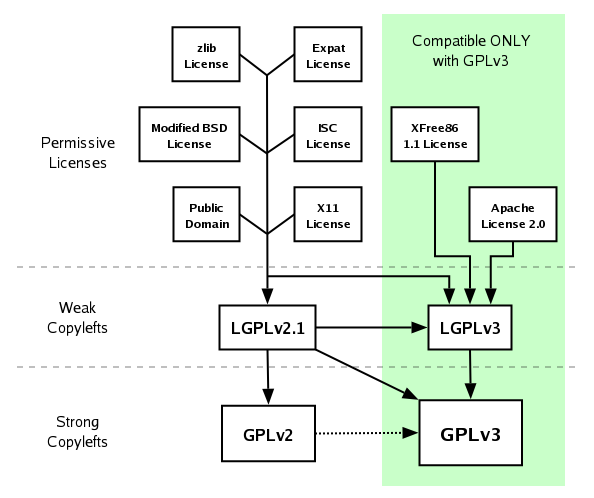
\includegraphics[width=.6\textwidth]{compatibility.png}
  \caption{GPL compatibility matrix. Note that GPL 3 is
    GPL 2-incompatible. Figure from \url{http://www.gnu.org/licenses/quick-guide-gplv3.html}.}
  \label{fig:compatibility}
\end{figure}

\subsection{Linking and copyright}

What is the effect in copyright law of linking against a library? Is the
resulting program a single work which contains both the program and the
library, or are the program and library separate works in object form even
when combined together? Perhaps surprisingly, there does not seem to be any
case law on this question, however many legal authors have considered this
question, especially in the context of the GPL. 

The question of linking, and dynamic linking\footnote{Dynamic linking in
  this context might be understood as extending to other run-time linking
  operations such as those that occur in Java and in interpreted languages
  such as Python.} in particular, arises in the context of the GPL because
the FSF asserts that if a GPL library is linked against a program, then
binary redistribution of that program is only possible under the
GPL\footnote{See, for example,
  \url{http://www.gnu.org/licenses/gpl-faq.html\#LinkingWithGPL}}. This
creates issues for, for example, the authors of proprietary binary-only
Linux kernel modules, such as the NVIDIA graphics driver.

The majority position among legal writers appears to be that dynamically
linking against a library does not infringe the copyright in that library,
and therefore the licence of the library is not relevant to the licence on
the main program\footnote{See, for example,
  \citet{Katz2007,Rosen2004,Lindberg2008}. The latter works are American but
  the arguments presented do not appear to rely on any aspect of copyright
  law which differs between the UK and the US.}. Here I will just briefly survey
the arguments for this. As a concrete example, have in mind the
classic C situation in which there is a library compiled as a shared object
(Linux \texttt{.so}, Windows \texttt{.dll}),
accompanying headers which define data structures and function prototypes,
and a main program which is to be compiled using those header files and
linked dynamically against the library at run time. 

Is the source code of the main program an adapation or copy of a substantial part of the
library? The only part of the library which is reproduced in the source code
is the names of the functions and external variables which are used in the
main program. Under \textit{SAS Institute Inc. v World Programming}, these
are functional, interface components which are not protected by
copyright. It is therefore difficult to see a basis on which the main
program source code could be found to infringe the copyright of the library
(and therefore be affected by the licence terms on the library).

Now consider the compiled binary main program, on disk and therefore not
currently linked against the library. This contains a translation of the
source code and the header files. As noted above, the source code is not
affected by the copyright in the library but the header files are directly
taken from the library. It now matters what is in those header files:
suppose they are typical C header files and only contain interface
information such as function prototypes and simple type declarations. The
ruling in \textit{SAS Institute Inc. v World Programming} would once again
appear to indicate that there is no copyright protection for these sorts of
header files. On this basis, the binary contains no copyright protected
material from the library, and so distribution of this binary would not
infringe copyright. The final point in the chain is the execution of the
program, at which point the dynamic linker matches the memory copy of the
executable with the memory copy of the library. \emph{If}\ this is
considered by a court to create a new work in the computer's memory, then
this might potentially infringe copyright (by making an adaptation of the
library) but the Software Directive\footnote{Art 5.1} makes it clear that
copies made in order to run the program do not infringe copyright in the
absence of licence terms to the contrary, and the GPL explicitly does not
place any restrictions on the running of software\footnote{GPL v3 clause
  2.}.

\subsection{Code in headers and static linking}

The arguments above can be generalised to a wide variety of circumstances:
including for interpreted and byte-compiled languages. However there are
some circumstances which are a little different from the dynamic linking
situation. First, if the program is statically linked rather than
dynamically linked, then the compiled code of the library is included in the
compiled binary program, and so copying the binary outside the terms of the
library licence will infringe copyright. In this circumstance it seems
likely that the GPL licence on the library does make distribution of the
binary program only possible if the program is released under GPL-compatible
terms.

Another similar situation occurs where the header files contain executable
code as well as interface information. If this executable code has
sufficient expressive quality that it is covered by copyright then use of
the headers is similar to the static compilation situation: the compiled
binary contains the compiled header code and therefore must comply with its
licence. 

\section{Further reading}

A leading UK text on digital copyright generally, including much more than
copyright in software, is \citet{Stokes2009}. A comprehensive, although US law-based, guide to
working with copyright and patent in an open source context is provided in
\citet{Lindberg2008}. Informative discussion of the
development of copyright law in the digital context is to be found in \citet{Lessig2006}.

\bibliography{bibliography}

\end{document}
* What is copyright? What rights and restrictions does it impose? Who owns the copyright in a work?
* Copyright as a form of intellectual property
* The scope of copyright in software: source code, object code and linking. 
* Limits to copyrightability: the idea/expression dichotomy and its impact in software. Can copyright cover languages and interfaces? 
* Software licenses, especially open source licenses. A brief overview of the most important open source licenses will be included.